\documentclass{beamer}
\usetheme{metropolis}
\usepackage{float}
\usepackage{listings}
\usepackage{xcolor}
\usepackage{transparent}
\usepackage{wasysym}

\definecolor{codegreen}{rgb}{0,0.6,0}
\definecolor{codegray}{rgb}{0.5,0.5,0.5}
\definecolor{codepurple}{rgb}{0.58,0,0.82}
% \definecolor{backcolour}{rgb}{0.95,0.95,0.95}
\definecolor{backcolour}{rgb}{0.98,0.98,0.98}

\lstdefinestyle{mystyle}{
    backgroundcolor=\color{backcolour},   
    commentstyle=\color{codegreen},
    keywordstyle=\color{magenta},
    numberstyle=\tiny\color{codegray},
    stringstyle=\color{codepurple},
    basicstyle=\ttfamily\fontsize{7}{5}\selectfont
    aboveskip=15pt, % Adjust the space above the listing
    belowskip=15pt, % Adjust the space below the listing
    breakatwhitespace=false,         
    breaklines=true,                 
    captionpos=b,                    
    keepspaces=true,                 
    numbers=left,                    
    numbersep=5pt,                  
    showspaces=false,                
    showstringspaces=false,
    showtabs=false,                  
    tabsize=1
}

\lstset{style=mystyle}

% \AtBeginSection[]
% {
%   \begin{frame}
%     \frametitle{Table of Contents}
%     \tableofcontents[currentsection]
%   \end{frame}
% }

\title{"mdmon" - Multiple Device Monitoring}
\subtitle{Laboratorio di Amministrazione di Sistemi}
\author{Gabriele Aloisio [503264]}

\institute{Università degli studi di Messina}
\date{2023}
\logo{
\includegraphics[height=1cm]{unime.png}}

\begin{document}
\maketitle

\begin{frame}{Table of contents}
    \tableofcontents
\end{frame}

\section{Introduction}
\begin{frame}{Descrizione del progetto}
    Il nostro progetto si focalizza sulla progettazione e implementazione di un'infrastruttura di storage basata su RAID in un ambiente operativo Linux. La configurazione di tale sistema prevede l'utilizzo di \textbf{RAID 1} (OS) e \textbf{RAID 5} (directory condivisa con \textbf{SAMBA}). Viene successivamente configurata la gestione degli accessi, consentendo agli utenti di accedere esclusivamente alle cartelle condivise. In fine, al fine di garantire una pronta risposta a eventuali guasti dei dischi, abbiamo implementato un sistema di alert. Questo sistema avverte gli amministratori di sistema tramite e-mail in caso di malfunzionamenti.
\end{frame}

\begin{frame}{RAID}
    Il RAID, acronimo di \textit{Redundant Array of Independent Disks}, è una tecnologia di archiviazione che combina più dischi rigidi in un'unica unità logica. L'obiettivo principale è migliorare la prestazione e/o fornire ridondanza dei dati per aumentare l'affidabilità e la sicurezza del sistema di storage.
\end{frame}

\begin{frame}{Tipologie di RAID}
    Nel contesto specifico del nostro progetto, implementeremo due livelli di RAID:

    \begin{itemize}
        \item \textbf{RAID 1:} In una configurazione RAID 1, due dischi rigidi contenenti gli stessi dati sono utilizzati in parallelo. Ogni dato scritto su un disco viene duplicato sull'altro, creando una copia identica.

        \item \textbf{RAID 5:} Nel caso di RAID 5, la ridondanza dei dati viene ottenuta mediante la distribuzione delle informazioni di parità su tutti i dischi del RAID array. Questo schema permette al sistema di recuperare i dati in caso di guasto di uno dei dischi.
    \end{itemize}
\end{frame}

\begin{frame}{Debian}
    Debian è un sistema operativo open-source basato su Linux, rinomato per la sua stabilità, affidabilità e flessibilità, ed è supportato da una vasta comunità di sviluppatori e utenti appassionati. È una scelta popolare per una varietà di utilizzi, dalle implementazioni di server aziendali alle soluzioni personalizzate. Grazie al suo \textit{package manager} \textbf{APT}, gli utenti possono facilmente installare, aggiornare e gestire le applicazioni con pochi comandi. Debian è particolarmente adatto per coloro che cercano un sistema operativo stabile e altamente personalizzabile.
\end{frame}

\begin{frame}{XFCE}
    Come ambiente desktop, abbiamo optato per \textbf{XFCE} per la sua leggerezza e semplicità. \textbf{XFCE} offre un'esperienza utente intuitiva senza compromettere le risorse di sistema, il che è importante per garantire prestazioni ottimali in ambienti server. La combinazione di \textbf{Debian} e \textbf{XFCE} ci fornisce un sistema stabile, facile da gestire e ottimizzato per le nostre esigenze di progetto.
\end{frame}

\begin{frame}{Cron}
    Cron è un servizio in ambiente Unix e Unix-like che consente agli utenti di programmare l'esecuzione automatica di comandi o script a intervalli specifici di tempo, giorni della settimana o mesi. In merito al progetto, utilizzeremo cron per automatizzare l'esecuzione periodica dello script \textbf{mdmon}. Questo script è progettato per monitorare lo stato dei dischi in un array RAID e inviare notifiche agli amministratori in caso di anomalie o malfunzionamenti.
\end{frame}

\begin{frame}{SAMBA}
    SAMBA è una suite di software che facilita l'integrazione di sistemi basati su Linux e Windows in una rete. Con \textbf{SAMBA}, è possibile condividere file e risorse tra piattaforme eterogenee. \textit{SAMBA} permette agli utenti di accedere a cartelle condivise, stampanti e altri servizi, con sicurezza e controllo degli accessi.
\end{frame}

\begin{frame}{Postfix}
    Postfix è un server di trasferimento di posta (MTA) utilizzato per la gestione dell'invio e della ricezione delle email in un sistema Linux. Nel contesto del nostro progetto, utilizzeremo Postfix per l'autenticazione e il relay delle email tramite il server SMTP di Google. Ciò significa che Postfix fungerà da intermediario tra il nostro sistema e il server SMTP di Google per inviare le email.
\end{frame}

\section{Debian e RAID}
\begin{frame}{Installazione di Debian su RAID1}
    L'installer ci permette comodamente di configurare la partizione \textbf{RAID 1} per il mountpoint di root (/) prima ancora di installare Debian. Il processo utilizzato è il seguente:
\end{frame}

\begin{frame}{Processo di configurazione RAID1}
    \begin{enumerate}
        \item Creare due partizioni vuote per \texttt{vda} e \texttt{vdb}
        \item Impostare il tipo delle partizioni come \textit{volume fisico per RAID}
        \item Creare un \texttt{MD} (multiple device) di tipo RAID1 (\texttt{md0})
        \item Impostare il numero di device attivi a 2
        \item Impostare il numero di spare device a 0
        \item Selezionare i device da utilizzare per l'array RAID1 (\texttt{vda1} e \texttt{vdb1})
        \item Creare Il filesystem di root sulla partizione RAID1 appena creata
    \end{enumerate}

\end{frame}

\begin{frame}[fragile]{mdadm}
Installiamo \texttt{mdadm} con
\begin{verbatim}
$ sudo apt update
$ sudo apt install mdadm -y
\end{verbatim}
\end{frame}

\begin{frame}[fragile]{Formattazione dischi}
Sucecssivamente formattiamo e partizioniamo i dischi \texttt{vdc}, \texttt{vdd} e \texttt{vde} con \texttt{fdisk}
\tiny\begin{lstlisting}
    Command (m for help): n
    Partition type
       p   primary (0 primary, 0 extended, 4 free)
       e   extended (container for logical partitions)
    Select (default p): p
    [...]
    Command (m for help): t
    Selected partition 1
    Hex code (type L to list all codes): fd
    Changed type of partition 'Linux' to 'Linux raid autodetect'.
    
    Command (m for help): w
    The partition table has been altered.
    Calling ioctl() to re-read partition table.
    Syncing disks.
    \end{lstlisting}
\end{frame}

\begin{frame}[fragile]{Configurazione di RAID5}
Creiamo l'array RAID5
\begin{verbatim}
$ mdadm --create /dev/md1 --level=5 
> --raid-devices=3 /dev/vdc /dev/vdd /dev/vde
\end{verbatim}
Ed un filesystem \texttt{ext4}
\begin{verbatim}
$ mkfs.ext4 /dev/md1
\end{verbatim}
Lo montiamo con
\begin{verbatim}
$ mount /dev/md1 /share
\end{verbatim}
E rendiamo la configurazione persistente inserendo questa voce in \texttt{/etc/fstab}
\begin{verbatim}
/dev/md1      /share     ext4   defaults        0 0
\end{verbatim}
\end{frame}

\begin{frame}[fragile]{Persistenza del nome del device}
Per default, RAID non dispone di un file di configurazione e quindi dobbiamo salvarlo manualmente. Se questo passaggio non viene seguito, il dispositivo RAID potrebbe essere denominato in un modo diverso da \texttt{md1}. Quindi, è necessario salvare la configurazione affinché persista tra i riavvii; quando avviene un riavvio, viene caricata nel kernel e il RAID viene anch'esso caricato:

\begin{verbatim}
$ mdadm --detail --scan --verbose >> /etc/mdadm.conf
\end{verbatim}
\end{frame}

\section{SAMBA}
\begin{frame}[fragile]{Installazione di SAMBA}
Installiamo SAMBA
\begin{verbatim}
$ sudo apt install samba
\end{verbatim}
E aggiungiamo il mountpoint \texttt{/share} in \texttt{/etc/samba/smb.conf}, specificando che gli utenti facenti parte del gruppo \texttt{sambashare} possono accedere alla directory:
\begin{lstlisting}
[share]
    comment = Samba shared directory
    path = /share
    read only = no
    browsable = yes
    valid users = @sambashare
\end{lstlisting}
\end{frame}

\begin{frame}[fragile]{Riavvio servizio}
Concludiamo riavviando il servizio
\begin{verbatim}
$ sudo systemctl restart smbd.service
\end{verbatim}
\end{frame}

\section{Creazione e configurazione dell'utenza}

\begin{frame}[fragile]{Creazione utenza}
Per dimostrare il funzionamento dei permessi della shared directory, creiamo due utenti \textit{user1} e \textit{user2}, dove solo \textit{user1} farà parte del gruppo \textit{sambashare}:
\begin{verbatim}
$ sudo useradd -m user1
$ sudo useradd -m user2
$ sudo groupadd sambashare
$ sudo usermod -aG sambashare user1
\end{verbatim}
\end{frame}

\begin{frame}[fragile]{Utenti}
Avremo quindi
\begin{verbatim}
$ groups user1
user1 : user1 users sambashare
$ groups user2
user2 : user2 users
\end{verbatim}
\end{frame}


\section{Sistema di alert}

\begin{frame}[fragile]{Script mdmon}
Lo script vero e proprio \texttt{/etc/cron.hourly/mdmon} viene eseguito ogni ora da \textit{cron}. Questo script legge un altro file di testo \texttt{/home/admin/fault\_msg} dove scriveremo il messaggio che \textbf{mdmon} invierà al destinatario. Un file di log \texttt{/var/log/mdmon.log} viene creato, dove si tiene traccia dei \textit{check} che esegue \textit{mdmon}. Il \textit{check} funziona controllando l'output del comando \texttt{mdadm --detail <dispositivo md>}, controllando con \texttt{awk} se lo stato è \textbf{degraded}. In questo caso, viene subito inviata una mail con il comando \texttt{mail} di \texttt{gnumail}.
\end{frame}

\begin{frame}[fragile]{checkmd.sh}
\begin{lstlisting}[language=Bash]
    #!/bin/bash
    
    log_file="/var/log/mdmon.log"
    fault_msg="/home/admin/fault_msg"
    recipient="example@mail.com"
        
    echo "$(date):" >> $log_file
        
    for i in /dev/md/*
    do
        state=$(sudo mdadm --detail $i | grep State | head -n 1 | awk '{print $NF}')
        if [[ $state = "degraded" ]]
        then
            mail -s "Degraded RAID partition ${i}" $recipient < $fault_msg
            echo "${i} faulty. Sent notification to administrator." >> $log_file
        else
            echo "${i} ok." >> $log_file
        fi
    done
        
    echo "" >> $log_file
        
    \end{lstlisting}
\end{frame}

\begin{frame}[fragile]{fault\_msg}
\begin{lstlisting}
This is an automated notification.

Dear Administrator,
This message was sent because one of the RAID partitions is in a degraded state.
It is suggested to intervene.
    
Sincerely,
The automated notification system
\end{lstlisting}
\end{frame}

\section{Installazione e configurazione di Postfix}
\begin{frame}[fragile]{Installazione Postfix}
Installiamo Postfix con
\begin{verbatim}
$ sudo apt install mailutils
\end{verbatim}
\end{frame}

\begin{frame}[fragile]{main.cf}
Configuriamo Postfix aggiungendo delle opzioni per l'autenticazione e il nostro relayhost al file \texttt{/etc/postfix/main.cf}:
\begin{lstlisting}[]
smtpd_relay_restrictions = permit_mynetworks permit_sasl_authenticated defer_unauth_destination
myhostname = labbox.org
alias_maps = hash:/etc/aliases
alias_database = hash:/etc/aliases
myorigin = /etc/mailname
mydestination = localhost.labbox.org, , localhost
relayhost = [smtp.gmail.com]:587
mynetworks = 127.0.0.0/8 [::ffff:127.0.0.0]/104 [::1]/128
mailbox_size_limit = 0
recipient_delimiter = +
inet_interfaces = all
inet_protocols = all
    
smtp_sasl_auth_enable = yes
smtp_sasl_security_options = noanonymous
smtp_sasl_password_maps = hash:/etc/postfix/sasl/sasl_passwd
smtp_tls_security_level = encrypt
smtp_tls_CAfile = /etc/ssl/certs/ca-certificates.crt
\end{lstlisting}
\end{frame}

\begin{frame}[fragile]{sasl\_passwd}
Creiamo il file delle credenziali \texttt{/etc/postfix/sasl/sasl\_passwd} e scriviamo dentro
\begin{verbatim}
[smtp.gmail.com]:587 example@email.com:<tua password>
\end{verbatim}
Con \texttt{postmap} possiamo convertire il file appena creato in un database
\begin{verbatim}
$ sudo postmap /etc/postfix/sasl/sasl_passwd
\end{verbatim}
Questo creerà un file \texttt{sasl\_passwd.db} nella stessa directory.
\end{frame}

\begin{frame}[fragile]{Permessi e riavvio}
Cambiamo i permessi del file per permettere solo all'utente \textit{root} di leggere e scrivere
\begin{verbatim}
$ sudo chown root:root /etc/postfix/sasl/sasl_passwd
$ sudo chmod 600 /etc/postfix/sasl/sasl_passwd
\end{verbatim}
Infine riavviamo il servizio Postfix
\begin{verbatim}
$ sudo systemctl restart postfix
\end{verbatim}
\end{frame}

\begin{frame}[fragile]{Permessi server di posta}
Bisognerà poi accedere al \textbf{pannello di controllo dell'account Google} per permettere ad "app meno sicure" di eseguire l'accesso.
\end{frame}

\section{Conclusioni}
\begin{frame}[fragile]{Conclusioni}
    Lo script funziona come previsto: nel caso di un malfunzionamento dei dischi \textbf{md} verrà inviata una mail all'indirizzo specificato nel file di configurazione e scritta una voce nel file di log. In caso contrario, cron continuerà ad eseguire lo script indefinitivamente, continuando a scrivere log sul file apposito.
\end{frame}

\begin{frame}[fragile]{Posta in arrivo}
    \begin{figure}[H]
        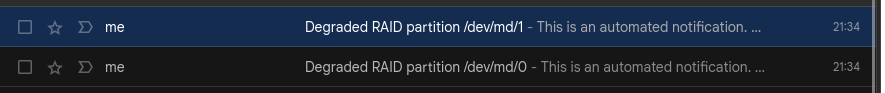
\includegraphics[width=0.8\textwidth, keepaspectratio]{../img/inbox.png}
        \centering
    
        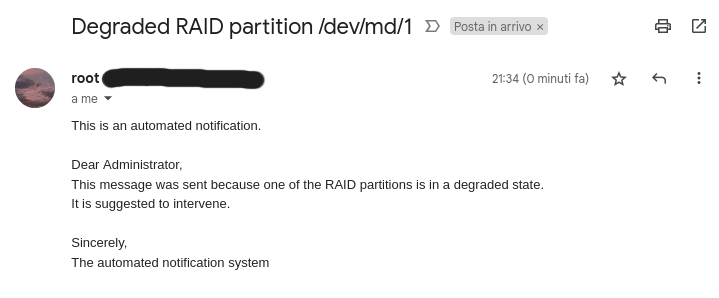
\includegraphics[width=0.8\textwidth, keepaspectratio]{../img/mail.png}
        \centering
    \end{figure}
\end{frame}

\begin{frame}[fragile]{File di log}
    \begin{figure}[H]
        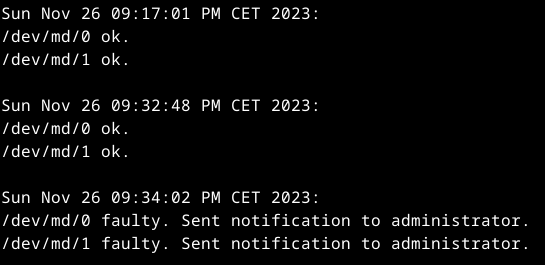
\includegraphics[width=0.8\textwidth, keepaspectratio]{../img/log.png}
        \centering
    \end{figure}
\end{frame}

\begin{frame}[standout]
    Grazie mille
    \\
    \Huge\smiley{}
\end{frame}

\end{document}